\documentclass[rgb]{beamer}

\usepackage[english]{babel}
\usepackage[utf8]{inputenc}
\usepackage{xcolor}
\usepackage{listings}
\usepackage{adjustbox}
\usepackage{amsmath}
\usepackage{multirow}
\usepackage[linewidth=1pt]{mdframed}

% Graphics
\usepackage{graphicx}

\usepackage{tikz}
\usetikzlibrary{calc,shapes.multipart,chains,arrows}

% Font
\usepackage{paratype}
\setbeamerfont{frametitle}{family=\bf}

% Beamer theme settings
\usecolortheme{seagull}
\setbeamertemplate{itemize item}{\raisebox{0.8mm}{\rule{1.8mm}{1.2mm}}}
\usenavigationsymbolstemplate{} % no navigation buttons

\usepackage{listings}

% Define Language
\lstdefinelanguage{fsharp}
{
  % list of keywords
  morekeywords={
    and,
    do,
    else,
    exception,
    for,
    fun,
    function,
    if,
    in,
    let,
    match,
    module,
    mutable,
    open,
    of,
    rec,
    then,
    try,
    type,
    unsafe,
    use,
    val,
    when,
    while,
    with,
  },
  sensitive=true, % keywords are not case-sensitive
  morecomment=[l]{//}, % l is for line comment
%  otherkeywords={>,<,=,<=,>=,!,*,/,-,+,|,&,||,&&,==,=>},
  morestring=[b]" % defines that strings are enclosed in double quotes
}

% Define Colors
\usepackage{color}
\definecolor{eclipseBlue}{RGB}{42,0.0,255}
\definecolor{eclipseGreen}{RGB}{63,127,95}
\definecolor{eclipsePurple}{RGB}{127,0,85}

\newcommand{\fop}[1]{\mbox{\ttfamily\color{eclipseBlue}#1}}
\newcommand{\fw}[1]{\mbox{\ttfamily\bfseries\color{eclipsePurple}#1}}

% Set Language
\lstset{
  language={fsharp},
  basicstyle=\ttfamily, % Global Code Style
  captionpos=b, % Position of the Caption (t for top, b for bottom)
  extendedchars=true, % Allows 256 instead of 128 ASCII characters
  tabsize=2, % number of spaces indented when discovering a tab
  columns=fixed, % make all characters equal width
  keepspaces=true, % does not ignore spaces to fit width, convert tabs to spaces
  showstringspaces=false, % lets spaces in strings appear as real spaces
  breaklines=true, % wrap lines if they don't fit
  frame=trbl, % draw a frame at the top, right, left and bottom of the listing
  frameround=tttt, % make the frame round at all four corners
  framesep=4pt, % quarter circle size of the round corners
  numbers=left, % show line numbers at the left
  numberstyle=\small\ttfamily, % style of the line numbers
  commentstyle=\slshape\bfseries\color{eclipseGreen}, % style of comments
  keywordstyle=\bfseries\color{eclipsePurple}, % style of keywords
  stringstyle=\color{eclipseBlue}, % style of strings
  emph=[1] {
    false,
    true,
    Set,
    Map,
    List,
    ImgUtil,
    Pegs,
    String,
    Array,
    Array2D
  },
  emphstyle=[1]{\color{eclipseBlue}},
  moredelim=**[is][\color{red}]{@@}{@@}
}

\newcommand{\theyear}{2020}
\newcommand{\sem}[1]{[\![#1]\!]}
\newcommand{\seme}[1]{\sem{#1}\varepsilon}
\newcommand{\semzero}[1]{\sem{#1}_0}

\newcommand{\emptymap}{\{\}}
\newcommand{\fracc}[2]{\begin{eqnarray} \frac{\begin{array}{c} #1
    \end{array}}{\begin{array}{c} #2 \end{array}} \end{eqnarray}}
\newcommand{\sembox}[1]{\hfill \normalfont \mbox{\fbox{\(#1\)}}}
\newcommand{\sempart}[2]{\subsubsection*{\rm\em #1 \sembox{#2}}}
\newcommand{\axiom}[1]{\begin{eqnarray} \begin{array}{c} #1 \end{array} \end{eqnarray}}
\newcommand{\fraccn}[2]{\refstepcounter{equation}\mbox{$\frac{\begin{array}{c} #1 \end{array}}{\begin{array}{c} #2 \end{array}}$}~(\arabic{equation})}
\newcommand{\fraccc}[2]{\mbox{$\frac{\begin{array}{c} #1 \end{array}}{\begin{array}{c} #2 \end{array}}$}}
\newcommand{\onepart}[1]{\noindent\hfill#1\hfill~\vspace{2mm}}
\newcommand{\twopart}[2]{\noindent\hfill#1\hfill#2\hfill~\vspace{2mm}}
\newcommand{\threepart}[3]{\noindent\hfill#1\hfill#2\hfill#3\hfill~\vspace{2mm}}
%\newcommand{\axiomm}[1]{\refstepcounter{equation}\mbox{$\begin{array}{c} #1 \end{array}$}~(\arabic{equation})}
\newcommand{\axiomm}[1]{$\begin{array}{c} #1 \end{array}$}
%\newcommand{\ar}[1]{\stackrel{#1}{\longrightarrow}}
\newcommand{\vd}{\vdash}
\newcommand{\Ran}{{\rm Ran}}
\newcommand{\Dom}{{\rm Dom}}
\newcommand{\kw}[1]{\texttt{#1}}
\newcommand{\id}[1]{\mbox{\it{#1}}}
\newcommand{\rarr}{\rightarrow}
\newcommand{\eval}{\rarr}
\newcommand{\evals}{\leadsto}
\newcommand{\larr}{\leftarrow}

\newcommand{\head}[1]{\vspace{3mm} \textbf{\normalsize #1}}
\newcommand{\headsp}[1]{\head{#1}\vspace{1ex}}
\newcommand{\size}{\ensuremath{\mathrm{size}}}
\renewcommand{\log}{\ensuremath{\mathrm{log}}}

\newcommand{\setallthemecolors}[1]{%
\setbeamercolor*{palette primary}{use=structure,fg=white,bg=#1}%
\setbeamercolor*{palette secondary}{use=structure,fg=white,bg=#1}%
\setbeamercolor*{palette tertiary}{use=structure,fg=white,bg=#1}}

\definecolor{black}{RGB}{0,0,0}
\definecolor{maroon}{RGB}{128,0,0}
\definecolor{olive}{RGB}{128,128,0}
\definecolor{green}{RGB}{0,128,0}
\definecolor{purple}{RGB}{128,0,128}
\definecolor{teal}{RGB}{0,128,128}
\definecolor{darkteal}{RGB}{0,92,92}
\definecolor{navy}{RGB}{0,0,128}
\definecolor{gray}{RGB}{128,128,128}
\definecolor{darkgray}{RGB}{60,60,60}
\definecolor{darkred}{RGB}{139,0,0}

%palette

% #173F5F (dark blue)
\definecolor{darkblue}{RGB}{23,63,95}
% #20639B (blue)
\definecolor{blue}{RGB}{32,99,155}
% #3CAEA3 (green)
\definecolor{magenta}{RGB}{60,174,163}
% #F6D55C (yellow)
\definecolor{yellow}{RGB}{246,213,92}
% #ED553B (red)
\definecolor{red}{RGB}{237,85,59}


\usecolortheme{whale}
\useoutertheme{infolines}
\useinnertheme{rectangles}

\newcommand{\popsettitle}[2]{%
\setallthemecolors{#1}%
\newcommand{\popemne}{#2}%
\title{Programmering og Problemløsning}%
\subtitle{#2}%
\author{Martin Elsman}%
\date{}%
\institute[DIKU]{Datalogisk Institut, Københavns Universitet (DIKU)}}

\newcommand{\popmaketitleframe}{%
  \frame{\titlepage%
   \vspace{-15mm}%
   \par\noindent\rule{\textwidth}{0.4pt}%

   \vspace{4mm}%
   \tableofcontents%
   \vspace{-4mm}%
   \par\noindent\rule{\textwidth}{0.4pt}%
  }%
  \section*{\popemne}%
}


\popsettitle{purple}{Typer og Mønstergenkendelse (Del 3)}  % see ../util.tex for colors

\begin{document}

\popmaketitleframe

%%%%%%%%%%%%%%%%%%%%%%%%%%%%%%%%%%%%%%%%%%%%%%%%
%\subsection{Introduktion}
%%%%%%%%%%%%%%%%%%%%%%%%%%%%%%%%%%%%%%%%%%%%%%%%

\begin{frame}[fragile]
\begin{footnotesize}

  \head{Sum-Typer}

  \vspace{1ex}
  Vi skal her se på begrebet sum-typer, som er grundlaget for at
  definere en lang række data-strukturer, såsom træer.

  \vspace{1ex}

  Vi har allerede set eksempler på sum-typer, som inkluderer lister og
  option-typer.

  \vspace{1ex}

  Sammen med basale datatyper som strenge, heltal og floats og sammen
  med typer for tupler, records og arrays giver sum-typer os et
  \textbf{komplet væktøjssæt} til at bygge datastrukturer og store
  applikationer.

  \vspace{1ex}

\begin{minipage}[b]{0.6\textwidth}

  \begin{enumerate}
  \item \textbf{Simple sum-typer (enumerations).}

  \item \textbf{Sum-typer med konstruktører der bærer argumenter.}

  \item \textbf{Generiske sum-typer.}

  \item \textbf{Mønstergenkendelse (pattern matching) for sum-typer.}
  \end{enumerate}
\end{minipage} \hspace{5mm}
\begin{minipage}[b]{0.3\textwidth}

  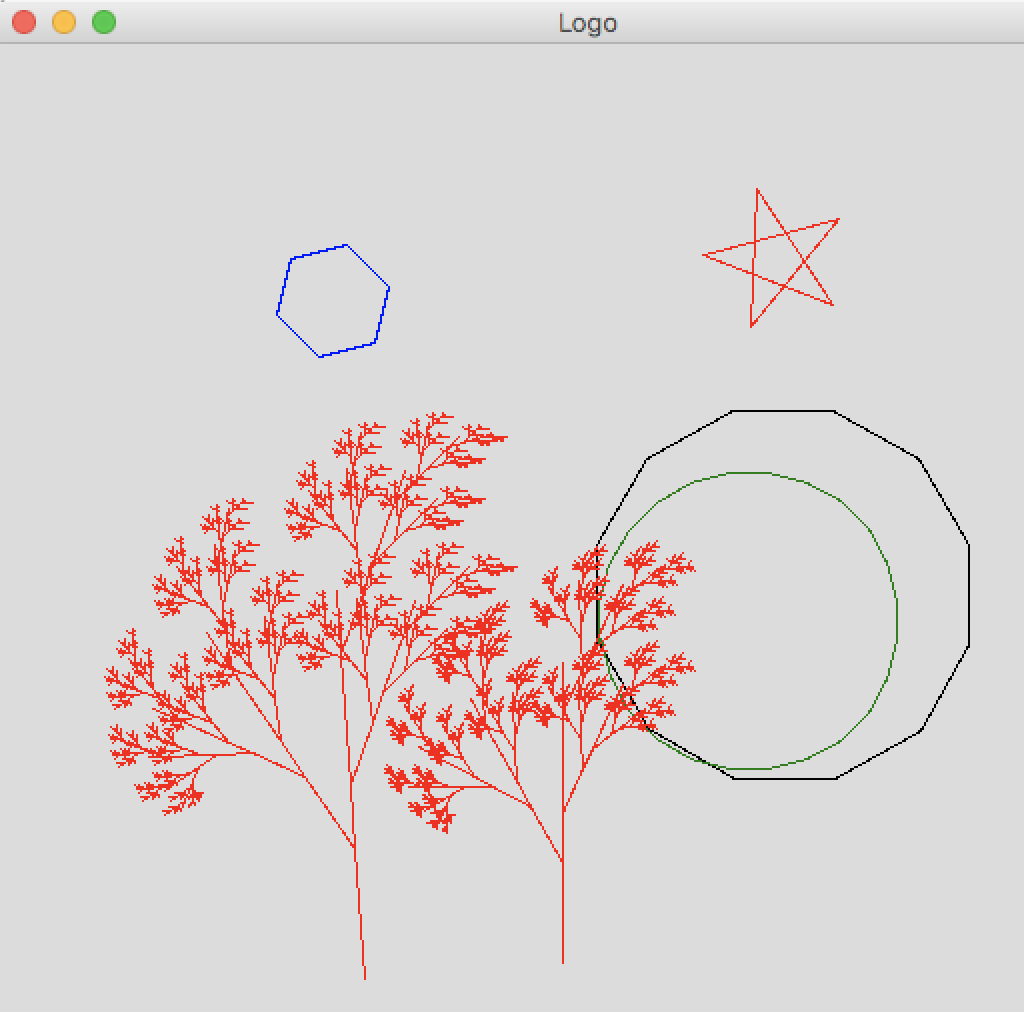
\includegraphics[width=\textwidth]{../images/turtle.png}

\end{minipage}

\end{footnotesize}
\end{frame}


\subsection{Simple sum-typer}
\begin{frame}[fragile]
\begin{footnotesize}

  \head{Simple sum-typer}
  \vspace{1ex}

  Det er nemt i F\# at erklære en sum-type bestående af en mindre mængde af ``tokens''.

  \vspace{1ex}

  \head{Eksempler:}
\begin{lstlisting}[numbers=none,frame=none,mathescape]
  type country = DK | UK | DE | SE | NO
  type currency = DKK | EUR | USD | CHF | GBP
  type direction = North | South | East | West
\end{lstlisting}

  \vspace{1ex}
  \head{Pattern-matching:}

\begin{lstlisting}[numbers=none,frame=none,mathescape]
  let opposite (dir:direction) : direction =
    match dir with
      | North -> South    // A constructor can appear
      | South -> North    // both as a pattern and as
      | East -> West      // an expression (just as
      | West -> East      // integers can)
\end{lstlisting}

\head{Bemærk:}
\begin{itemize}
\item Det kan være en fordel at benytte sig af simple sum-typer i
  stedet for f.eks. streng- eller heltals-repræsentationer af data.
\end{itemize}

\end{footnotesize}
\end{frame}

\subsection{Sum-typer med argument-bærende konstruktører}
\begin{frame}[fragile]
\begin{footnotesize}

  \head{Sum-typer med argument-bærende konstruktører}
  \vspace{1ex}

  Sum-typer kan have konstruktører der tager argumenter.

  \vspace{1ex}

  \head{Eksempel:}

\begin{lstlisting}[numbers=none,frame=none,mathescape]
  type obj = Pnt | Circ of float | Rect of float * float
\end{lstlisting}

  \vspace{1ex}
  \head{Pattern-matching er nu mulig:}
\begin{lstlisting}[numbers=none,frame=none,mathescape]
  let rec area (obj:obj) : float =
    match obj with
    | Pnt -> 0.0
    | Circ r -> System.Math.PI * r * r
    | Rect (a,b) -> a * b
\end{lstlisting}

  \vspace{1ex}

\head{Bemærk:}
\begin{itemize}
\item Det er ikke et krav at alle konstruktører tager argumenter; \lstinline{Pnt} tager ikke et argument.
\item Konstruktører der tager argumenter virker som funktioner i udtryk; f.eks. har \lstinline{Circ} typen \lstinline{float -> obj}.
\end{itemize}

\end{footnotesize}
\end{frame}

\subsection{Generiske sum-typer}
\begin{frame}[fragile]
\begin{footnotesize}

  \head{Sum-typer kan være type-generiske.}
  \vspace{1ex}

  Sum-type definitioner kan være \emph{generiske} således at de er
  parameteriserede over en eller flere typer.

  \vspace{1ex}

  Denne mulighed kan være brugbar til at skabe genbrugelige konstruktioner.

  \vspace{1ex}

\head{Option-typen er et godt eksempel:}

\begin{lstlisting}[numbers=none,frame=none,mathescape]
  type 'a option = None | Some of 'a
\end{lstlisting}

  \vspace{1ex}
  \head{Vi kan nu skrive generisk (genbrugelig) kode:}
\begin{lstlisting}[numbers=none,frame=none,mathescape]
  let valOf (default:'a) (obj:'a option) : 'a =
    match obj with
    | None -> default
    | Some v -> v
\end{lstlisting}

  \vspace{1ex}

\head{Spørgsmål:}
\begin{itemize}
\item Nævn en anden type-generisk sum-type?
\end{itemize}

\end{footnotesize}
\end{frame}


\begin{frame}[fragile]
\begin{footnotesize}

  \head{Sum-typer er et meget kraftigt redskab}
  \vspace{1ex}

  Sum-typer åbner op for en lang række muligheder:
  \vspace{1ex}
  \begin{itemize}
  \item Sum-typer kan moduleres med produkter (tupler), men giver
    mulighed for en mere præcis definition af data-sammenhænge.
  \vspace{1ex}
  \item Sum-typer baner vejen for let at definere såkaldte ``embeddede''
    domain-specifikke sprog (EDSLs).
  \vspace{1ex}
  \item Sammen med pattern-matching giver sum-typer beriget kontrol
    over at alle kode-tilfælde er håndteret (jvf. \lstinline{area} funktionen).
  \end{itemize}

  \vspace{1ex}

  \head{Rekursivt-definerede sum-typer}
  \vspace{1ex}
  \begin{itemize}
  \item Lister kan (som nævnt) forstås som en generisk rekursivt-defineret sum-type med to konstruktører (\lstinline{[]} og \lstinline{::}).
\begin{lstlisting}[numbers=none,frame=none,mathescape]
  type 'a list = [] | (::) of 'a * 'a list
\end{lstlisting}
  \item Vi skal senere se hvorledes vi også kan definere mere avancerede generiske data-strukturer, såsom træer, ved hjælp af generiske rekursive sum-typer.
  \end{itemize}

\end{footnotesize}
\end{frame}

\subsection*{Konklusion}
\begin{frame}[fragile]
  \headsp{Konklusion}

  \vspace{3mm}
  \tableofcontents
\end{frame}

\end{document}

\subsection{Eksempel: Skildpadde EDSL}

\begin{frame}[fragile]
\begin{footnotesize}

  \head{Eksempel: Skildpadde EDSL}
  \vspace{1ex}

  Som et illustrativt eksempel vil vi se på at definere et
  skildpaddesprog til brug for at tegne \textbf{skildpaddegrafik} (kendt fra
  programmeringssprog som \textbf{Logo}).

  \vspace{1ex}

  \head{Ide:}
  \begin{itemize}
  \item Definer et sprog der kan specificere en skildpaddes bevægelser (gå et antal skridt frem, roter et antal grader).
  \item Giv samtidig mulighed for at skildpadden kan tegne med en pen
    i en given farve (skildpadden skal kunne skifte pen samt løfte
    pennen op og ned).
  \end{itemize}

  \head{Simpelt domain-specifikt sprog (DSL) som sum-type i F\#:}

\begin{lstlisting}[numbers=none,frame=none,mathescape]
type cmd =              // turtle command
  | SetColor of color     // change pen color
  | Turn of int           // degrees right (0-360)
  | Move of int           // 1 unit = 1 pixel
  | PenUp                 // avoid drawing when moving
  | PenDown               // draw when moving
\end{lstlisting}

\end{footnotesize}
\end{frame}

\begin{frame}[fragile]
\begin{footnotesize}

  \head{Eksempler på skildpaddebevægelser}
  \vspace{1ex}

  Lad os først antage at vi har en måde hvorpå vi kan ``oversætte''
  en liste af skildpaddebevægelser til et billede.

  \vspace{1ex}

\begin{minipage}[b]{0.7\textwidth}

  \head{Skildpaddegrafik:}
  \vspace{1ex}
\begin{lstlisting}[numbers=none,frame=none,mathescape]
  // Draw equal-sided triangle
  let triangle x =
    [Turn 30; Move x; Turn 120; Move x;
     Turn 120; Move x; Turn 90]

  // Define helper command to repeat
  // turtle commands
  let rec repeat n cmds =
    if n <= 0 then []
    else cmds @ repeat (n-1) cmds

  // Draw a star using 5 lines
  let star sz =
    repeat 5 [Move sz; Turn 144]
\end{lstlisting}
\end{minipage} \hspace{5mm}
\begin{minipage}[b]{0.2\textwidth}

  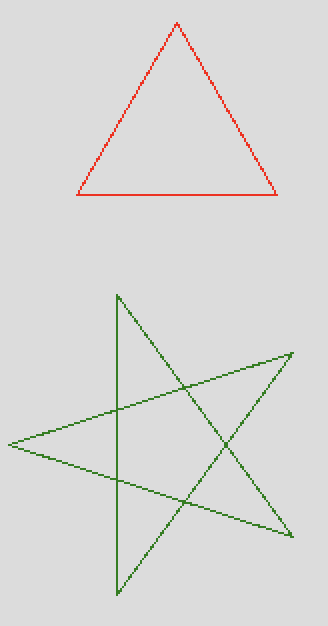
\includegraphics[width=\textwidth]{../images/turtle0.png}

\end{minipage}

\end{footnotesize}
\end{frame}


\begin{frame}[fragile]
\begin{footnotesize}

  \head{Fortolkning af Skildpaddekommandoer}
  \vspace{1ex}

  Før vi kan skrive en ``skildpaddekommandofortolker'' må vi først
  bestemme os for hvilke tilstande en skildpadde kan være i.

  \vspace{1ex}

  \head{Skildpaddetilstande:}
  \vspace{1ex}
  \begin{itemize}
  \item Position (type \lstinline{point = int*int}; initielt i midten af billedet)
  \item Retning (grader relativt til x-aksen: initielt $^\mathrm{o}$90).
  \item Farve (initielt sort på grå baggrund)
  \item Er pennen oppe eller nede (boolean; \lstinline{true} hvis oppe)
  \end{itemize}

  \vspace{1ex}
  Vi skal også bestemme os for hvad resultatet af ``fortolkningen'' skal være.
  \vspace{1ex}

  Hvis vi nu kunne fortolke kommandoerne til en \textbf{liste af
  linier} (af type \lstinline{point*point*color}) vil vi kunne benytte os af
  \lstinline{ImgUtil.setLine} til at tegne linierne på et bitmap:
\begin{lstlisting}[numbers=none,frame=none,mathescape]
val setLine : color -> int*int -> int*int -> bitmap -> unit
\end{lstlisting}

\end{footnotesize}
\end{frame}

\begin{frame}[fragile]
\begin{footnotesize}

  \head{Skildpaddekommandofortolkningen}
  \vspace{1ex}
\begin{lstlisting}[numbers=none,frame=none,mathescape]
type point = int * int
type line = point * point * color
let rec interp (p:point,d:int,c:color,up:bool) (cmds:cmd list) : line list =
  match cmds with
    | [] -> []
    | SetColor c :: cmds -> interp (p,d,c,up) cmds
    | Turn i :: cmds -> interp (p,d-i,c,up) cmds
    | PenUp :: cmds -> interp (p,d,c,true) cmds
    | PenDown :: cmds -> interp (p,d,c,false) cmds
    | Move i :: cmds ->
      let r = 2.0 * System.Math.PI * float d / 360.0
      let dx = int(float i * cos r)
      let dy = -int(float i * sin r)
      let (x,y) = p
      let p2 = (x+dx,y+dy)
      let lines = interp (p2,d,c,up) cmds
      if up then lines else (p,p2,c)::lines
\end{lstlisting}

\vspace{-25mm}\hspace{90mm}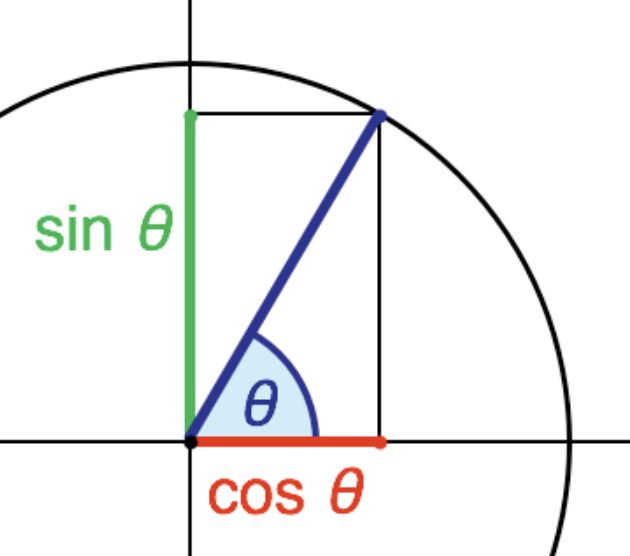
\includegraphics[width=25mm]{../images/cossin.png}

\end{footnotesize}
\end{frame}

\begin{frame}[fragile]
\begin{footnotesize}

  \head{Koden der tegner billedet og viser det i et vindue}
  \vspace{1ex}

\begin{lstlisting}[numbers=none,frame=none,mathescape]
let lightgrey = ImgUtil.fromRgb (220,220,220)
let black     = ImgUtil.fromRgb (0,0,0)

let draw (w,h) pic =
  let bmp = ImgUtil.mk w h
  for x in [0..w-1] do                       // initialize
    for y in [0..h-1] do                     // background
      ImgUtil.setPixel lightgrey (x,y) bmp
  let initState = ((w/2,h/2),90,black,false)
  let lines = interp initState pic           // run interp
  for (p1,p2,c) in lines do
    ImgUtil.setLine c p1 p2 bmp              // update bitmap
  ImgUtil.show "Logo" bmp                    // show bitmap
\end{lstlisting}

  \head{Bemærk:}
  \begin{itemize}
  \item Vi benytter os af to nestede for-løkker til at initialisere baggrunden.
  \item Vi benytter en for-in løkke samt
    \lstinline{setLine} til at tegne linierne på bitmap'et.
  \end{itemize}

\end{footnotesize}
\end{frame}

\begin{frame}[fragile]
\begin{footnotesize}

  \head{Træ-fraktalen med skildpaddegrafik}
  \vspace{1ex}

\begin{minipage}{0.68\textwidth}

\begin{lstlisting}[numbers=none,frame=none,mathescape]
let rec tree sz =
  if sz < 5 then
    [Move sz; PenUp; Move (-sz); PenDown]
  else
    [Move (sz/3);
     Turn -30] @ tree (sz*2/3) @ [Turn 30;
     Move (sz/6);
     Turn 25] @ tree (sz/2) @ [Turn -25;
     Move (sz/3);
     Turn 25] @ tree (sz/2) @ [Turn -25;
     Move (sz/6); PenUp;
     Move (-sz/3);   // not safe to
     Move (-sz/6);   // reduce these
     Move (-sz/3);   // moves to a
     Move (-sz/6);   // single move!
     PenDown]
\end{lstlisting}
\end{minipage}
\begin{minipage}{0.3\textwidth}

  ~\hspace{-5mm}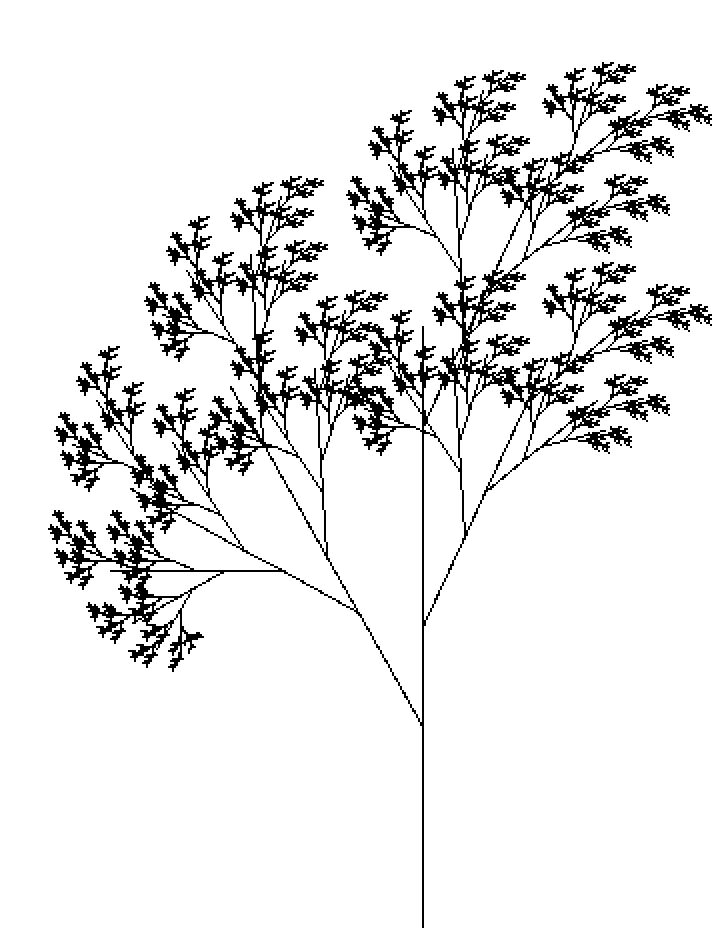
\includegraphics[width=1.2\textwidth]{../images/tree.png}

\end{minipage}

\vspace{1ex}
\textbf{Spørgsmål:} Hvorfor er det ikke en god ide at reducere de sidste fire
    \lstinline{Move} kommandoer til en enkelt \lstinline{Move}
    kommando?

\end{footnotesize}
\end{frame}


\end{document}


\begin{frame}[fragile]
\begin{footnotesize}

  \head{Type-generiske type-forkortelser}
  \vspace{1ex}

  Type-forkortelser kan være generiske således at det er muligt at
  skrive generisk kode der henviser til en type-forkortelse:

  \vspace{1ex}

\begin{lstlisting}[numbers=none,frame=none,mathescape]
  // association lists mapping strings to values of type 'a
  type 'a alist = (string * 'a) list
  let add (m:'a alist) (s:string) (v:'a) : 'a alist =
     (s,v)::m
  let rec look (m:'a alist) (s:string) : 'a option =
    if List.isEmpty m then None
    else if fst(List.head m) = s then Some(snd(List.head m))
         else look (List.tail m) s
  let empty () : 'a alist = []
\end{lstlisting}

  \head{Bemærk:}
  \begin{itemize}
  \item Vi kan benytte den tomme liste \lstinline{[]} til at repræsentere den tomme associationsliste.
  \item Vi skal senere se hvorledes vi med moduler kan sikre at typen
    \lstinline{'a alist} bliver ``fuldt abstrakt'' således at kun de
    nævnte funktioner kan benyttes til at opererere på de konstruerede
    associationslister.
  \end{itemize}

\end{footnotesize}
\end{frame}

\subsection{Records}

\begin{frame}[fragile]
\begin{footnotesize}

  \head{Record-typer}

  \vspace{1ex}

  Records i F\# giver mulighed for at navngive elementer i et tuple.

  \vspace{1ex}

  Syntaksen for at definere en record-type er ganske enkelt:

\begin{lstlisting}[numbers=none,frame=none,mathescape]
  type person = {first:string; last:string; age:int}

  let xs = [{first="Lene"; last="Andersen"; age=56};
            {last="Hansen"; first="Jens"; age=39}]
  let name (p:person) : string = p.first + " " + p.last
  let incr_age (p:person) : person = {p with age=p.age+1}
  let ys = List.map incr_age xs
\end{lstlisting}

  \vspace{1ex}

  \head{Bemærk:}
  \begin{itemize}
  \item Ved konstruktion af en record er felt-rækkefølgen ubetydelig.
  \item Elementer i en record kan udtrækkes ved brug af \textbf{dot-notationen} (\lstinline{p.first}).
  \item En \textbf{ny} record kan konstrueres (med et opdateret
    element) ved brug af \lstinline{with}-konstruktionen.
  \end{itemize}

\end{footnotesize}
\end{frame}

\subsection{Mønstergenkendelse}
\begin{frame}[fragile]
\begin{footnotesize}

  \head{Mønstergenkendelse (Pattern matching)}

  \vspace{1ex}

  Generelt set giver mønstergenkendelse mulighed for at \textbf{undersøge} og
  \textbf{nedbryde} en værdi i dens bestanddele.

  \vspace{1ex}

  Vi vil se på mønstergenkendelse ud fra typen på de værdier vi
  undersøger.

  \vspace{1ex}

  I F\# kan mønstergenkendelse optræde i flere forskellige programkonstruktioner:
  \begin{itemize}
  \item I simple \lstinline{let}-bindinger.
  \item I \lstinline{match-with}-konstruktioner.
  \item I funktionsparametre.
  \end{itemize}

\end{footnotesize}
\end{frame}

\begin{frame}[fragile]
\begin{footnotesize}

  \head{Mønstergenkendelse på Tupler}

    \vspace{1ex}

\begin{lstlisting}[numbers=none,frame=none,mathescape]
  let x = (34,"hej",2.3)    // construct triple
  let (_,b,f) = x           // use of wildcard (_)
  do printfn "%s:%f" b f    // b and f are available here
\end{lstlisting}

    \vspace{1ex}

  \head{Mønstergenkendelse på Records}

\begin{lstlisting}[numbers=none,frame=none,mathescape]
  type person = {first:string; last:string; age:int}
  let name ({first=f;last=l}:person) = f + " " + l
\end{lstlisting}

  \vspace{1ex}

  \head{Bemærk:}
  \begin{enumerate}
  \item Matching på records kræver blot at et udvalg af felt-navne er nævnt.
  \item Hvis flere record-typer benytter samme felt-navne kan det være nødvendigt med type-annoteringer.
  \item Mønstergenkendelse for tupler og records er også meget anvendte i funktionsparametre:
\begin{lstlisting}[numbers=none,frame=none,mathescape]
  let swap (x:'a,y:'b) : 'b * 'a = (y,x)
\end{lstlisting}
  \end{enumerate}

\end{footnotesize}
\end{frame}

\begin{frame}[fragile]
\begin{footnotesize}

  \head{Mønstergenkendelse på heltal og andre grundtyper}

  \vspace{1ex}

  Implementation af Fibonacci med mønstergenkendelse:

  \vspace{1ex}

\begin{lstlisting}[numbers=none,frame=none,mathescape]
  let rec fib n =
    match n with
    | 1 -> 1
    | 2 -> 1
    | _ -> fib(n-1) + fib(n-2)
  let v = fib 10
\end{lstlisting}

  \vspace{1ex}

  \head{Bemærk:}
  \begin{enumerate}
  \item Den første bar (\lstinline{|}) i en match-case er optional.
  \item Den første match-case der ``matcher'' vinder.
  \item Wildcards (\lstinline{_}) kan benyttes i en match-case.
  \item Tilsvarende kan der matches på andre grundtyper, såsom karakterer, booleans og strenge.
  \end{enumerate}
\end{footnotesize}
\end{frame}

\begin{frame}[fragile]
\begin{footnotesize}

  \head{Mønstergenkendelse på option-værdier}

  \vspace{1ex}

  Typen \lstinline{int option} er et eksempel på en simpel såkaldt
  ``sum-type'', også kaldt ``discriminated union'', som repræsenterer
  værdier der enten er værdien \lstinline{None} eller er en værdi
  \lstinline[mathescape]{Some($v$)}, hvor $v$ er en værdi af typen
  \lstinline{int}.

    \vspace{1ex}

  Her er en funktion der ``løfter'' addition til værdier af typen \lstinline{int option}:
\begin{lstlisting}[numbers=none,frame=none,mathescape]
  let add_opt (a:int option) (b:int option) : int option  =
    match a, b with
    | Some a, Some b -> Some(a+b)
    | _ -> None
\end{lstlisting}

  \head{Bemærk:}
  \begin{enumerate}
  \item Der benyttes her en form for ``nested pattern matching'' på
    par af værdier af typen \lstinline{int option}.
  \item Ved konstruktion og matching af tupler kan man ofte undvære brugen af parenteser.
  \item Variabler kan \textbf{bindes} i en match-case og henvises til i højre-siden af en match, hvor de vil varetage de matchede værdier.
  \end{enumerate}
\end{footnotesize}
\end{frame}


\begin{frame}[fragile]
\begin{footnotesize}

  \head{Mønstergenkendelse på lister}

  \vspace{1ex}

  Liste-værdier \textbf{konstrueres} grundlæggende set ved brug af to forskellige konstruktører:

  \vspace{1ex}
  \begin{tabular}{llp{7cm}}
    \texttt{[]} & (Nil) & Konstruktion af den tomme liste.  \\
    \texttt{x::xs} & (Cons) & Konstruktion af et listeelement med hovedet \texttt{x} og halen \texttt{xs} (en anden liste).
  \end{tabular}

  \vspace{1ex}

  Samme to konstruktorer benyttes ved mønstergenkendelse på en liste:
  \vspace{1ex}

\begin{lstlisting}[numbers=none,frame=none,mathescape]
  let rec length (l: 'a list) : int =
    match l with
    | [] -> 0
    | x::xs -> 1 + length xs
\end{lstlisting}

  \vspace{1ex}
  \head{Mønstergenkendelse med \lstinline{function}-konstruktionen}

\begin{lstlisting}[numbers=none,frame=none,mathescape]
  let rec length : 'a list -> int =
    function [] -> 0
           | x::xs -> 1 + length xs
\end{lstlisting}

\textbf{Bemærk:} Funktionsparameter og \lstinline{match-with}-konstruktionen sammentrækkes.

\end{footnotesize}
\end{frame}

\begin{frame}[fragile]
\begin{footnotesize}

  \head{Nestede mønstergenkendelser på lister}

  \vspace{1ex}

  Liste-værdier kan matches til dybere niveauer end første cons-celle:

    \vspace{1ex}

\begin{lstlisting}[numbers=none,frame=none,mathescape]
  let lengthy (l: 'a list) : bool =
    match l with
    | _::_::_ -> true  // at least two cells
    | _ -> false
\end{lstlisting}

    \vspace{1ex}

  Mønstre kan være mere komplekse:
  \vspace{1ex}
\begin{lstlisting}[numbers=none,frame=none,mathescape]
  let rec ones (l: int list) : int =
    match l with
    | [] -> 0
    | 1::xs -> 1 + ones xs  // match-cases are tested in order
    | _::xs -> ones xs
\end{lstlisting}

\end{footnotesize}
\end{frame}


\subsection{Selection Sort---genbesøgt}

\begin{frame}[fragile]
\begin{footnotesize}

  \head{Selection Sort---uden mønstergenkendelse}

  \begin{itemize}
  \item Udtræk det mindste element i listen.
  \item Gentag processen rekursivt indtil der ikke længere er elementer i listen.
  \end{itemize}

  \head{En implementation i F\#:}

\begin{lstlisting}[numbers=none,frame=none,mathescape]
let rec select (xs:int list) (m,ys) =
  if List.isEmpty xs then (m,ys)
  else let x = List.head xs
       let xs = List.tail xs
       in if x < m then
            if m <> System.Int32.MaxValue then
              select xs (x,m::ys)
            else select xs (x,ys)
          else select xs (m,x::ys)
let rec ssort xs =
  if List.isEmpty xs then xs
  else let (m,xs) = select xs (System.Int32.MaxValue,[])
       in m :: ssort xs
\end{lstlisting}

\end{footnotesize}
\end{frame}

\begin{frame}[fragile]
\begin{footnotesize}

  \head{Selection Sort---med mønstergenkendelse}

  \vspace{1ex}

  Ny implementation i F\#:

  \vspace{1ex}

\begin{lstlisting}[numbers=none,frame=none,mathescape]
let maxInt = System.Int32.MaxValue
let rec select (xs:int list) (m,ys) =
  match xs with
    | [] -> (m,ys)
    | x::xs -> if x < m then
                 if m <> maxInt then
                   select xs (x,m::ys)
                 else select xs (x,ys)
               else select xs (m,x::ys)
let rec ssort =
  function [] -> []
         | xs -> let (m,xs) = select xs (maxInt,[])
                 in m :: ssort xs
\end{lstlisting}
\end{footnotesize}
\end{frame}

\begin{frame}[fragile]
\begin{footnotesize}

\head{Analyse af Selection Sort --- Set tidligere}

\vspace{1ex}

\begin{minipage}[b]{0.55\textwidth}

  Funktionen \lstinline{select} køres $N$ gange og for hver kørsel
  gennemløbes listen (i gennemsnit $N/2$ elementer).

\vspace{1ex}

\head{Summary:}

\vspace{1ex}
  \begin{tabular}{ll}
    Best time: & $O(N^2)$ \\
    Worst time: & $O(N^2)$ \\
    Average time: & $O(N^2)$
  \end{tabular}

  \vfill
\mbox{ }
\end{minipage} \hspace{1cm}
\begin{minipage}[b]{0.3\textwidth}

  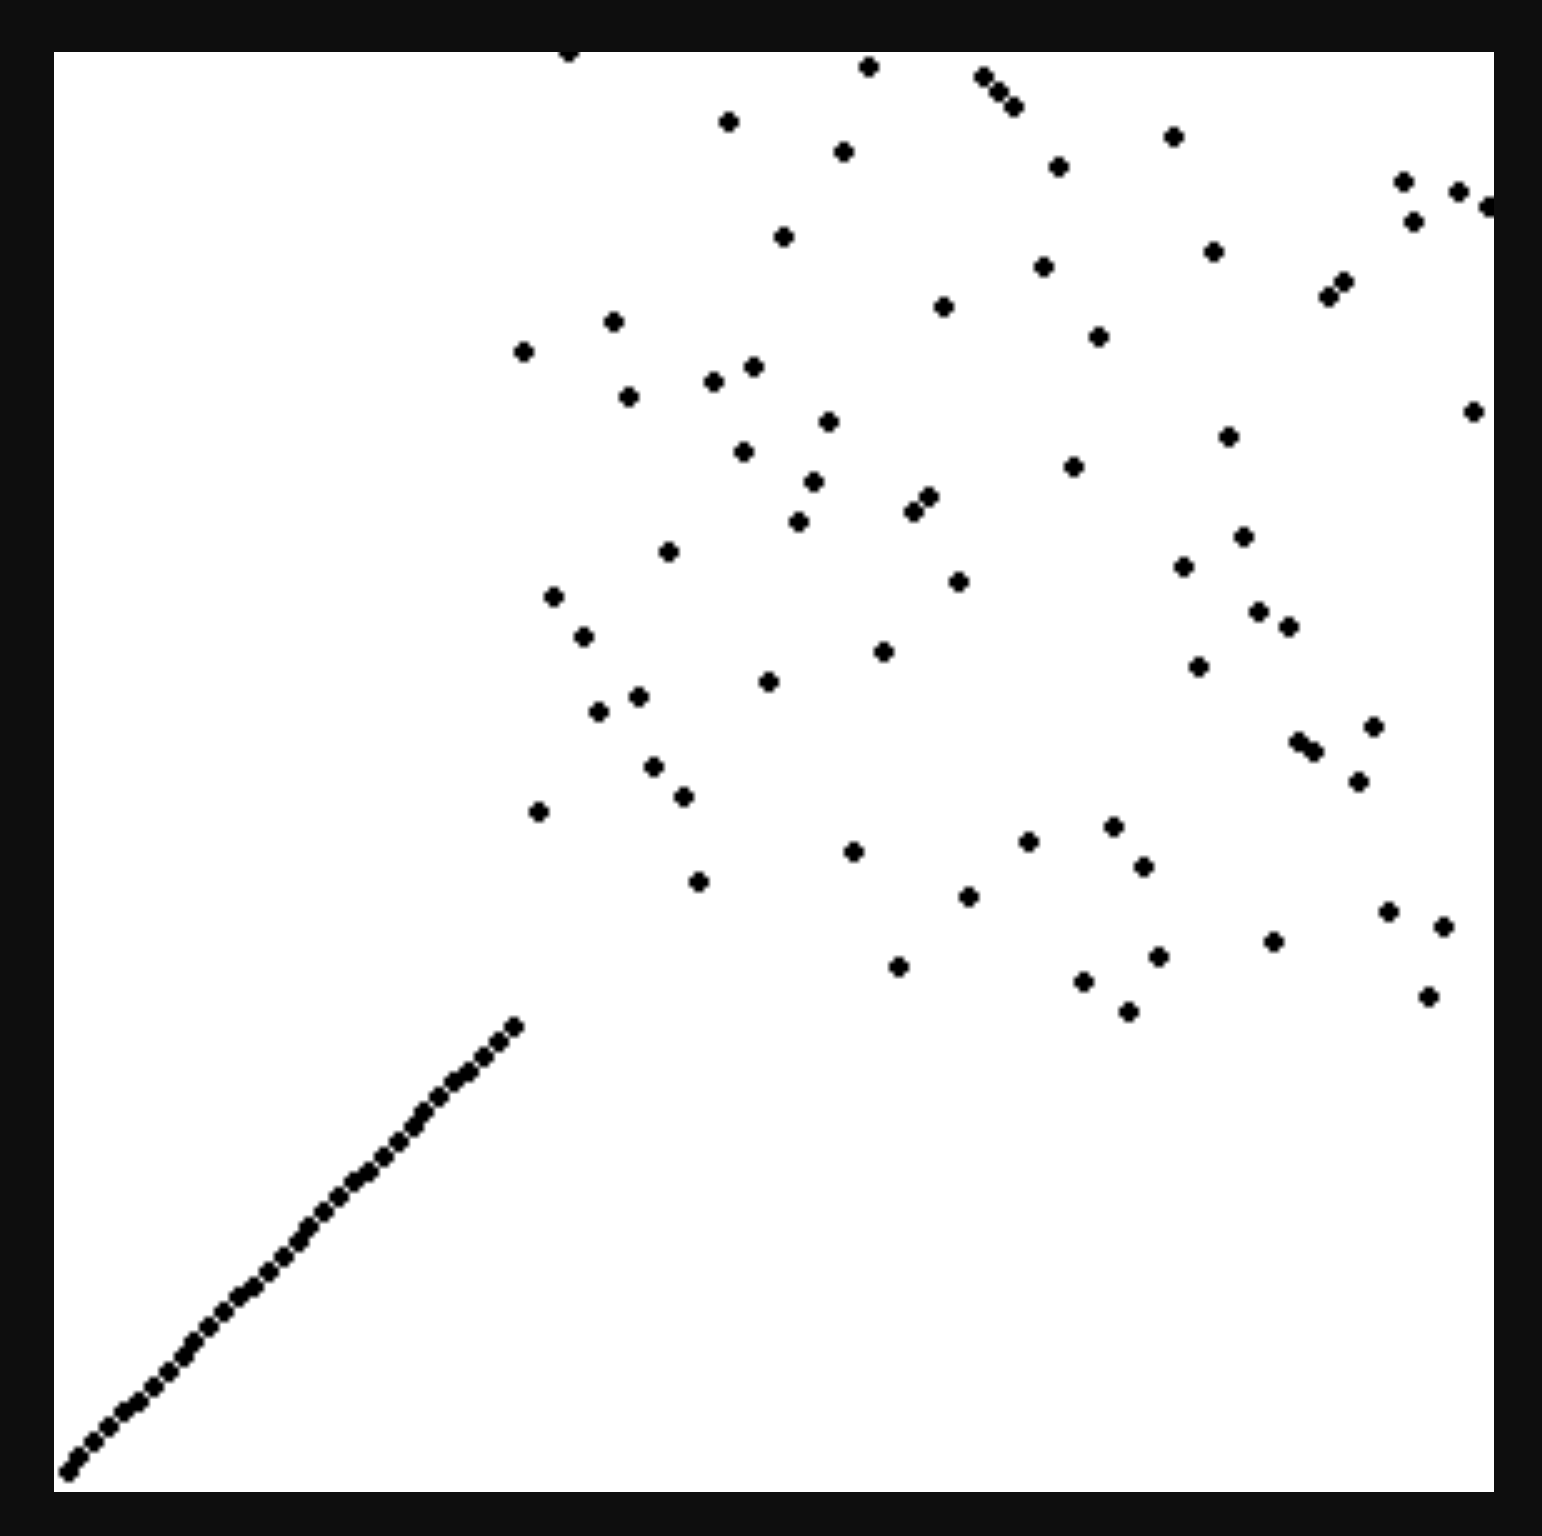
\includegraphics[width=\textwidth]{../images/ssort_gif.png}

  (\href{https://upload.wikimedia.org/wikipedia/commons/b/b0/Selection_sort_animation.gif}{animation})
\end{minipage}

\end{footnotesize}
\end{frame}

\end{document}
